\begin{refsection}[research/hirao/group.bib]
\nocite{*}
\chapter{Computational Chemistry Research Unit}

\section{Members}

\begin{itemize}
  \item[] Kimihiko Hirao (Unit Leader)
  \item[] Jong-Won Song (Research Scientist)
  \item[] Yukio Kawashima (Research Scientist)
  \item[] Sachiko Kikumoto (Assistant)
  \item[] Yumeno Kusuhara (Assistant)
  \item[] Takao Tsuneda (Senior Visiting Scientist)
  \item[] Bun Chan (Visiting Researcher)
\end{itemize}

\section{Research Activities}

Electronic structure calculations are now indispensible for understanding chemical phenomena. Density functional theory (DFT), which is simple, conceptual, and applicable to large systems, has emerged as a powerful computational tool to tackle molecular electronic structures. DFT efficiently calculates electronic structure with high accuracy, and its algorithm is suitable for parallel computing. DFT now plays an important role in applications of molecular science running on the K Computer. However, conventional DFT could not describe important properties such as van der Waals interaction and charge-transfer excitation, which are essential for accurate calculations for large-scaled molecular systems.\par
We have developed long-range corrected density functional theory (LC-DFT), which overcomes the drawbacks of conventional DFT mentioned above. LC-DFT also succeeded in describing induced/response properties. Recently, we found that LC-DFT obtains accurate energies of highest occupied molecular orbital (HOMO) and lowest occupied molecular orbital (HOMO). This indicates that prediction of chemical reactions can be done by LC-DFT calculations. The development of LC-DFT had a large impact in theoretical chemistry and the number of researches based on LC-DFT is growing intensively. However, LC-DFT has difficulty in describing photochemical reactions. Photochemical process includes avoided crossing among electronic states, spin-forbidden transitions, and states with high and low spins. These properties cannot be calculated accurately by LC-DFT. Moreover, the HF exact exchange, which remedies the shortcoming of the exchange functional in conventional DFT, requires large computational effort for real systems, which is the bottleneck for large-scale calculation. \par
The objective of our project is to establish LC-DFT to be a standard electronic structure theory by expanding its capability. We feature new developments of photo- and electro-chemical reaction theories and its high-speed computational algorithms for using on next-generation supercomputer “K”, and the elucidations of significant reaction mechanisms and the designs of new functional materials in photo and electrochemistry. We also aim to increase reliability of electronic structure calculation by improving the accuracy of LC-DFT. 


\section{Research Results and Achievements}
\subsection{Long-Range Corrected Density Functional Theory with Linearly-Scaled Hartree-Fock Exchange Using a Two-Gaussian Operator}
Hybrid density functionals have become a main quantum chemical tool for the calculation of energies and properties of molecular systems since its development in 1993. The Hartree-Fock (HF) exchange introduced in hybrid functionals remedy the shortcomings of density functional theory (DFT). Development of long-range corrected hybrid scheme for density functional theory, which follows a decade later, widened the applicability of the hybrid functional further. The introduction of the error function HF exchange operator in DFT calculation increased performance on orbital energy, excitation energy, non-linear optical property, barrier height, and so on. Nevertheless, the high cost associated with the evaluation of HF exchange integrals remain as a bottleneck for the broader and more active applications of hybrid functionals to large molecular and periodic systems. We proposed a very simple yet efficient method for the computation of long-range corrected hybrid scheme. It uses a modified two-Gaussian attenuating operator instead of the error function for the long-range HF exchange integral. As a result, the two-Gaussian HF operator, which mimics the shape of the error function operator, reduces computational time dramatically (e.g., about 14 times acceleration in C diamond calculation using periodic boundary condition) and enables lower scaling with system size, while maintaining the improved features of the long-range corrected density functional theory.

\begin{figure}[ht]
\centering
  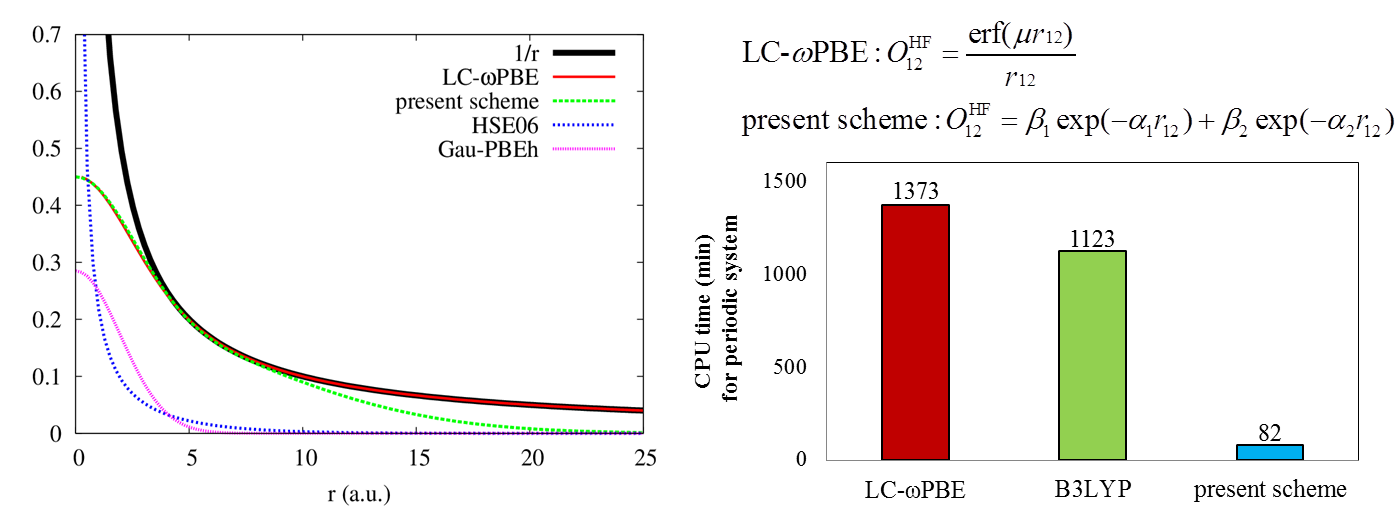
\includegraphics[width=0.9\textwidth,keepaspectratio,natwidth=193,natheight=40]
  {research/hirao/annual_hirao_2015_1.png}
  \caption{Functions of the HF exchange operator (left) and CPU time comparison of the new proposed method vs conventional methods (right). }
  \locallabel{fig:hirao-label1}
\end{figure}

\subsection{Development of efficient algorithm for Gaussian Hartree-Fock exchange operator}
Hybrid density functionals have succeeded in increasing the accuracy of density functional theory (DFT) by including Hartree-Fock (HF) exchange. Nowadays, most electronic structure calculations for isolated systems employ hybrid density functionals. Inclusion of HF exchange lead to improvement of electronic structure calculations for extended systems as well. The accuracy of bandgap, which is a major factor determinig electronic conductivity in extended systems, increased dramatically. However, the computational cost of HF exchange inhibits the use of hybrid density functionals for electronic structure calculations for extended or large-scale systems. We previously developed an efficient screened hybrid functional called Gaussian-Perdew–Burke–Ernzerhof (Gau-PBE) [Song et al., J. Chem. Phys. 135, 071103 (2011)], which is characterized by the usage of a Gaussian function as a modified Coulomb potential for the Hartree-Fock (HF) exchange. We found that the adoption of a Gaussian HF exchange operator considerably decreases the calculation time cost of periodic systems while improving the reproducibility of the bandgaps of semiconductors compared to previously developed well-known methods. We present a distance-based screening scheme here that is tailored for the Gaussian HF exchange integral that utilizes multipole expansion for the Gaussian two-electron integrals. We found the new multipole screening scheme saves the computational cost for the HF exchange integration by efficiently decreasing the number of integrals of the near field region without incurring substantial changes in total energy. In our assessment on the periodic systems of seven semiconductors, the Gau-PBE hybrid functional with a new screening scheme is 1.2 times faster than our previous implementation, and 2.1 times faster than the well-known HSE06 method.

\begin{figure}[ht]
\centering
  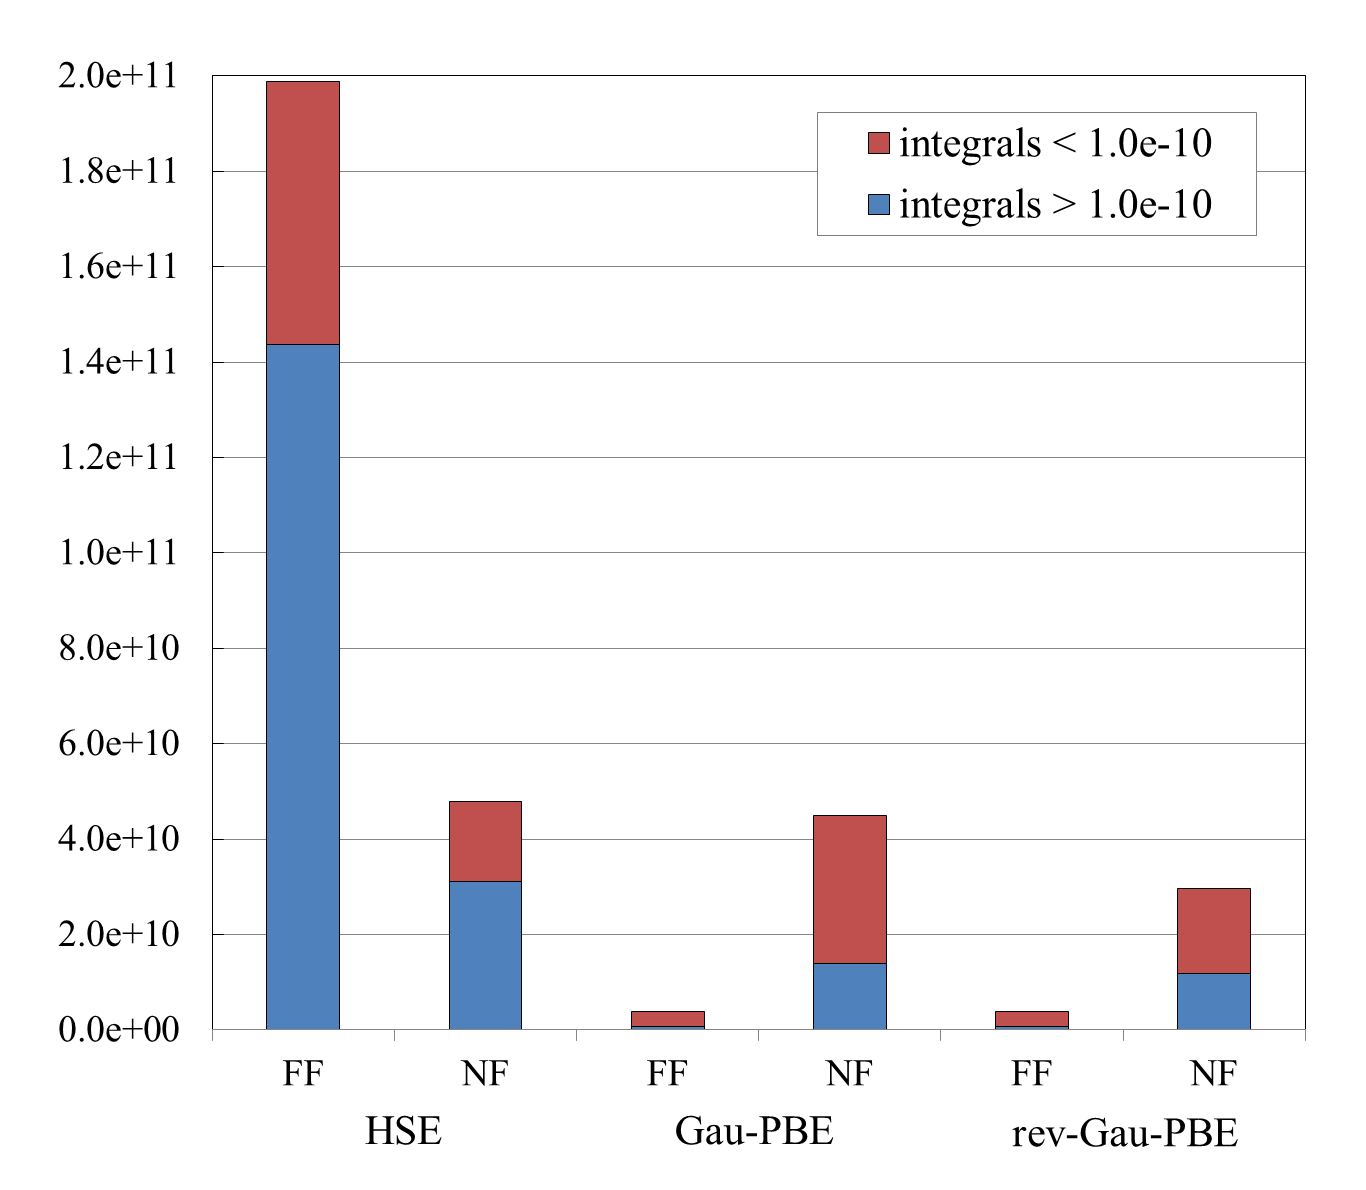
\includegraphics[width=0.7\textwidth,keepaspectratio,natwidth=193,natheight=40]
  {research/hirao/annual_hirao_2015_2.png}
  \caption{The numbers of calculated HF exchange integrals of HSE, Gau-PBE, and rev-Gau-PBE in C diamond.}
  \locallabel{fig:hirao-label2}
\end{figure}

\subsection{Critical Assessment of Same-Spin Correlation in OP Correlation Functional}
In the present study, we have investigated two significant features of the OP correlation functional, namely the incorporation of the exchange functional into itself, and the inclusion of only opposite-spin (OS) effects. To explore the latter feature, we have compared OP with B95 and a new functional introduced in the present study – the OPB method that combines OP with the same-spin (SS) component of B95. In general, we find that B95 and OPB perform comparably. Our comparisons of the various Density Functional Theory (DFT) procedures suggest that the incorporation of a meta-GGA (e.g., TPSS) into OP and OPB does not necessarily lead to a chemically more accurate procedure than the use of a related GGA (e.g., PBE). An important finding is the more notable (and somewhat more consistent) improvement in performance with the incorporation of SS correlation, particularly for longer-range chemical properties. Nonetheless, on average across our test sets of over 800 systems, the difference between the performances of OP versus B95 or OPB is not exceedingly large. By drawing a parallel between these DFT methods and the wavefunction scaled-MP2-type methods, we reason that one can further develop the OP functional, and perhaps a wider range of correlation functionals by combining it with the technique of range separation.

\subsection{Probing Fullerene Formation by Supercomputers}
Fullerenes are nano-sized carbon materials studied intensively due to its to its wide applicability such as a silver bullet for HIV, cosmetics, and superconductive devices. However, its precise value of ''heat of formation'', which is a fundamental property to understand how materials form and change, was not yet known. We have carried out large-scale computational quantum chemistry calculations on the K computer with NTChem software to obtain heats of formation for C$_{60}$ and some higher fullerenes with the DSD-PBE-PBE/cc-pVQZ double-hybrid density functional theory method. Our best estimated values are 2520.0 $\pm$ 20.7 (C$_{60}$), 2683.4 $\pm$ 17.7 (C$_{70}$), 2862.0 $\pm$ 18.5 (C$_{76}$), 2878.8 $\pm$ 13.3 (C$_{78}$), 2946.4 $\pm$ 14.5 (C$_{84}$), 3067.3 $\pm$ 15.4 (C$_{90}$), 3156.6 $\pm$ 16.2 (C$_{96}$), 3967.7 $\pm$ 33.4 (C$_{180}$), 4364 (C$_{240}$) and 5415 (C$_{320}$) kJ/mol. Using the convergence behavior for the calculated per-atom heats of formation, we obtained the formula $\Delta_{f}H$ per carbon = 722n$^{{-}0.72}$  + 5.2 kJ/mol (n  = the number of carbon atoms), which enables an estimation of $\Delta_{f}H$ for higher fullerenes more generally. A slow convergence to the graphene limit is observed, which we attribute to the relatively small proportion of fullerene carbons that are in “ low-strain” regions. We further propose that it would take tens, if not hundreds, of thousands of carbons for a fullerene to roughly approach the limit. Such a distinction may be a contributing factor to the discrete properties between the two types of nanomaterials. During the course of our study, we also observe a fairly reliable means for the theoretical calculation of heats of formation for medium-sized fullerenes. This involves the use of isodesmic-type reactions with fullerenes of similar sizes to provide a good balance of the chemistry and to minimize the use of accompanying species.
%
\begin{figure}[ht]
\centering
  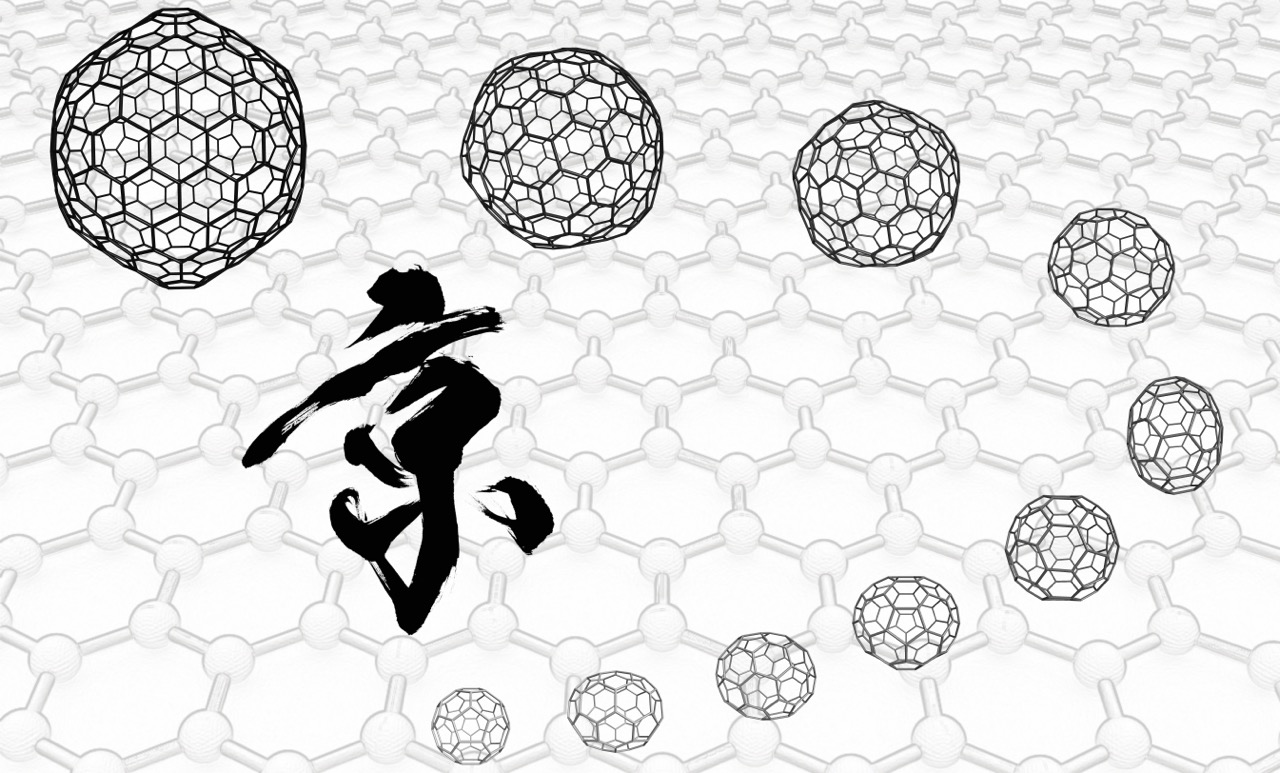
\includegraphics[width=0.5\textwidth,keepaspectratio,natwidth=193,natheight=40]
  {research/hirao/annual_hirao_2015_3.png}
  \caption{Illustration of fullerene systems calculated on the K computer.}
  \locallabel{fig:hirao-label3}
\end{figure}

%Text for research Results and achievements. Journal-artcile~\cite{sample-journal}.
%Conference-paper~\cite{sample-conference}.
%Invited-talk~\cite{sample-invited}.

%For cross referencing, use \verb|\locallabel| and \verb|\localref| to avoid conflicting names defined by other groups. For example, a figure can be referenced as Figure~\localref{fig:sample-label1}.

%\begin{figure}
%\centering
%  \includegraphics[width=0.5\textwidth,keepaspectratio,natwidth=193,natheight=40]
%  {sample_division/sample_group/test1.png}
%  \caption{Caption for a sample figure}
%  \locallabel{fig:sample-label1}
%\end{figure}

\section{Schedule and Future Plan}
We will continue our effort to expand the capabilities of LC-DFT. First, we will develop the order-N calculation algorithm of LC-DFT to calculate large molecular systems quantitatively with much less computational time. We have gained insight on how to reduce the time-consuming exact exchange calculation and we will apply our knowledge to the algorithm development. We will then apply this algorithm to excited state calculations on time-dependent density functional theory (TDDFT). We will also develop open-shell spin-orbit TDDFT to calculate molecular systems including metal atoms. Furthermore, we will develop a new method to calculate the nonadiabatic coupling among different electronic states, and carry out nonadiabatic coupling calculations based on TDDFT to reproduce photochemical reactions comprehensively. We are also planning to develop methods for solid-state calculations.

%%% DO NOT EDIT BELOW

\section{Publications}

%\printbibliography[keyword=journal, heading=subbibliography, title={Journal Articles}, prefixnumbers={1-}, resetnumbers=true]
%\printbibliography[keyword=proceedings, heading=subbibliography, title={Conference Papers}, prefixnumbers={2-}, resetnumbers=true]
%\printbibliography[keyword=invited, heading=subbibliography, title={Invited Talks}, prefixnumbers={3-}, resetnumbers=true]
%\printbibliography[keyword=poster, heading=subbibliography, title={Posters and Presentations}, prefixnumbers={4-}, resetnumbers=true]
%\printbibliography[keyword=deliverable, heading=subbibliography, title={Patents and Deliverables}, prefixnumbers={5-}, resetnumbers=true]

\printbibliography[keyword=journal, heading=subbibliography, title={Journal Articles}, resetnumbers=true]
\printbibliography[keyword=proceedings, heading=subbibliography, title={Conference Papers}]
\printbibliography[keyword=invited, heading=subbibliography, title={Invited Talks}]
\printbibliography[keyword=poster, heading=subbibliography, title={Posters and Presentations}]
\printbibliography[keyword=deliverable, heading=subbibliography, title={Patents and Deliverables}]

\end{refsection}
